\section{Results}

\subsection{Prior Results}

Earlier Fishery and Harvest results in the same project provide the empirical baseline. Fishery Commons provides the narrower signal-design result. In the matched baseline, monitoring with sanctions reduces held-out collapse relative to no governance under both mutation-based injection and live model-generated JSON strategy injection. In the broader non-LLM top-down sweep, adaptive quotas emerge as the strongest overall central signal in the medium tier, while temporary closures remain a credible ecological fallback.

Harvest Commons provides the stronger baseline architecture claim. In the restored four-condition pilot, bottom-up-only governance is empirically distinct from the no-governance baseline but remains ecologically weaker than architectures with central intervention. In the high-power confirmatory matrix, hybrid governance ranks first in all eight decision cells under the failure-then-patch-health-then-welfare rule. Relative to top-down-only governance, hybrid improves patch health in all eight cells, is non-worse on neighborhood overharvest in six of eight, and incurs a moderate mean welfare delta of \(-0.1363\). Relative to bottom-up-only governance, both architectures with central intervention buy large ecological gains at substantially larger welfare cost.

\begin{figure}[t]
  \centering
  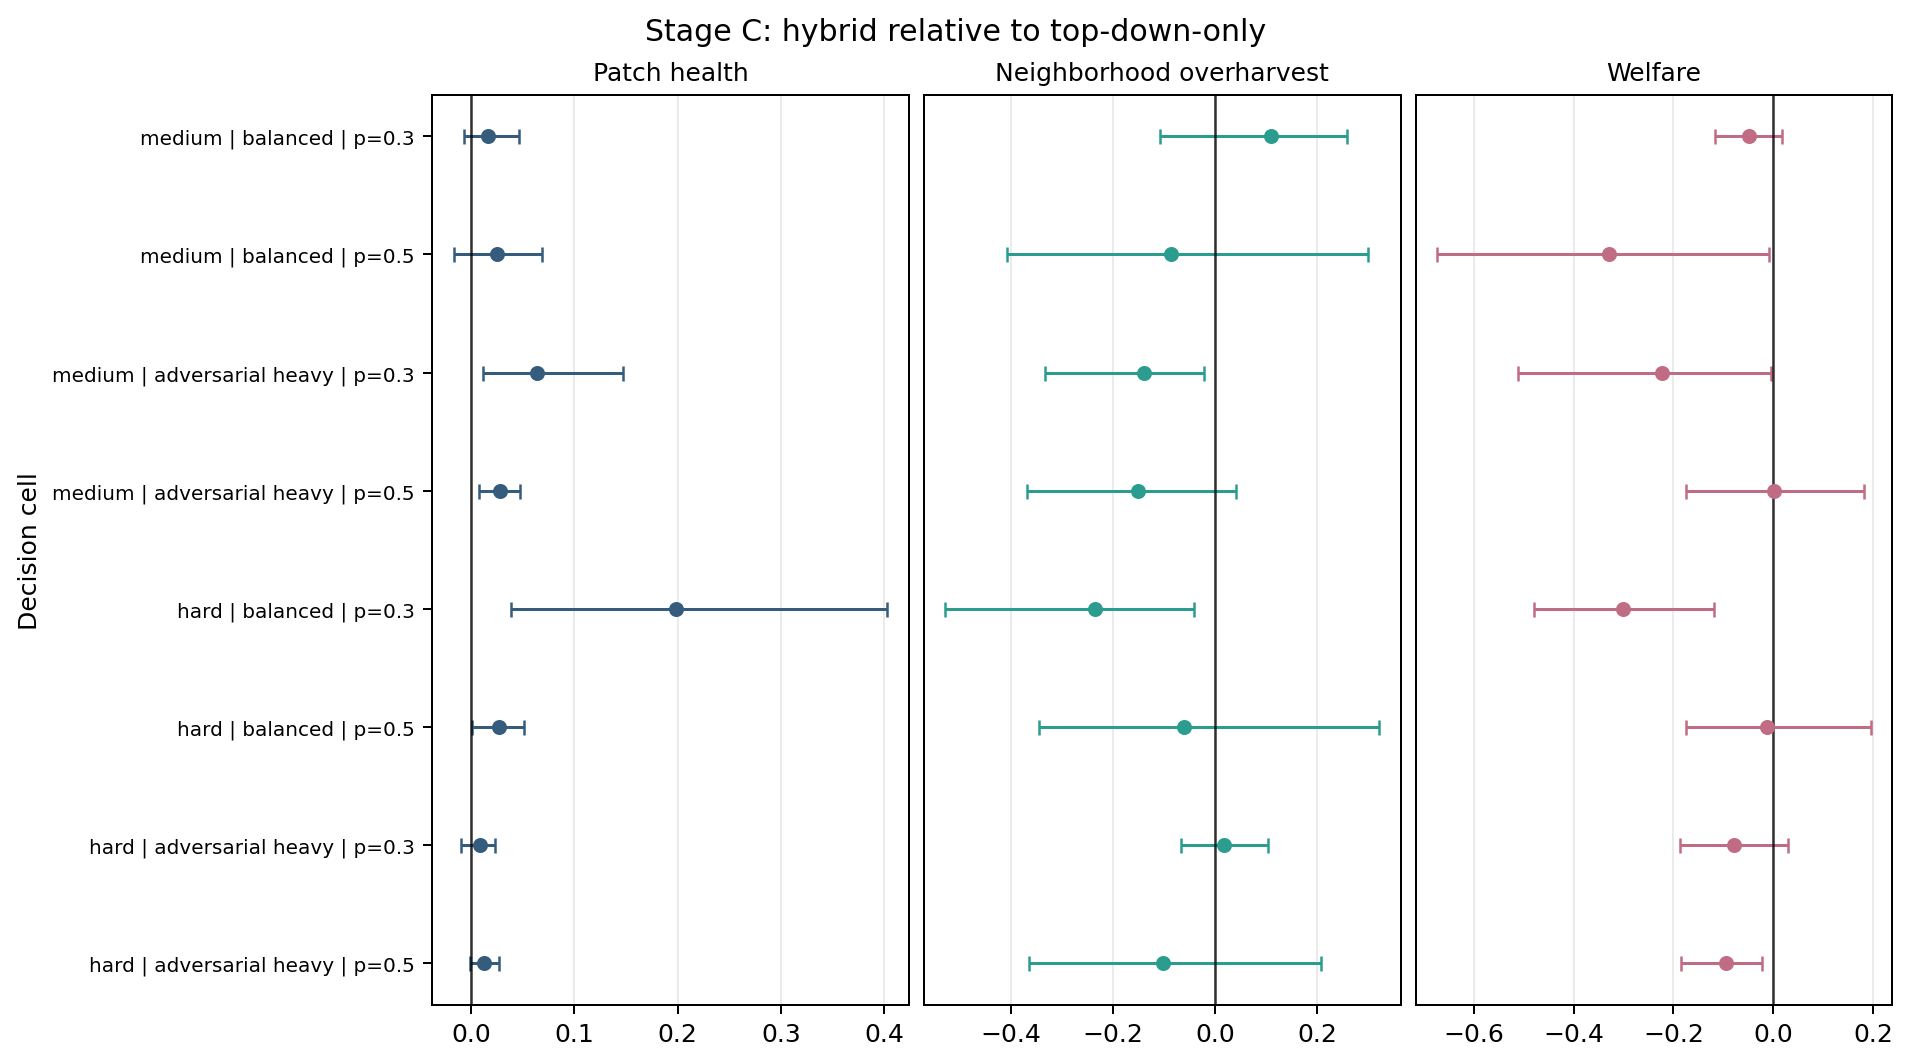
\includegraphics[width=\linewidth,trim={0 0 0 1.25cm},clip]{figures/harvest_architecture_stageC_architecture.png}
  \caption{Baseline Harvest architecture effect sizes from the confirmatory architecture matrix. Under the failure-then-patch-health-then-welfare rule, hybrid governance ranks first in all eight confirmatory cells while improving patch health in every cell relative to top-down-only control.}
  \label{fig:baseline_stagec_architecture}
\end{figure}

The capability ladder and welfare-incidence analyses sharpen that baseline result. Across the 32 ladder cells, hybrid governance ranks first in 25 and top-down-only governance ranks first in 7, while both governed architectures retain a stable ecological advantage over bottom-up-only governance throughout the non-LLM attacker ladder. The incidence summaries show that the additional welfare cost of moving from top-down-only to hybrid governance is modest relative to the much larger penalty associated with restoring ecological control over local-only governance. Figures~\ref{fig:baseline_stagec_architecture} and~\ref{fig:baseline_capability_ladder} are regenerated from the frozen result bundles used in the earlier studies.

Taken together, the carried-forward evidence establishes three points that matter for the extension. Fishery Commons shows that central interventions can be ranked under repeated strategic turnover. The confirmatory Harvest matrix provides a strong baseline result for hybrid governance before oversight frictions are introduced. The capability ladder and welfare-incidence analyses show that architectures with central intervention remain ecologically stronger than local-only governance even when the ordering between hybrid and top-down-only governance becomes more contested.

\begin{figure}[t]
  \centering
  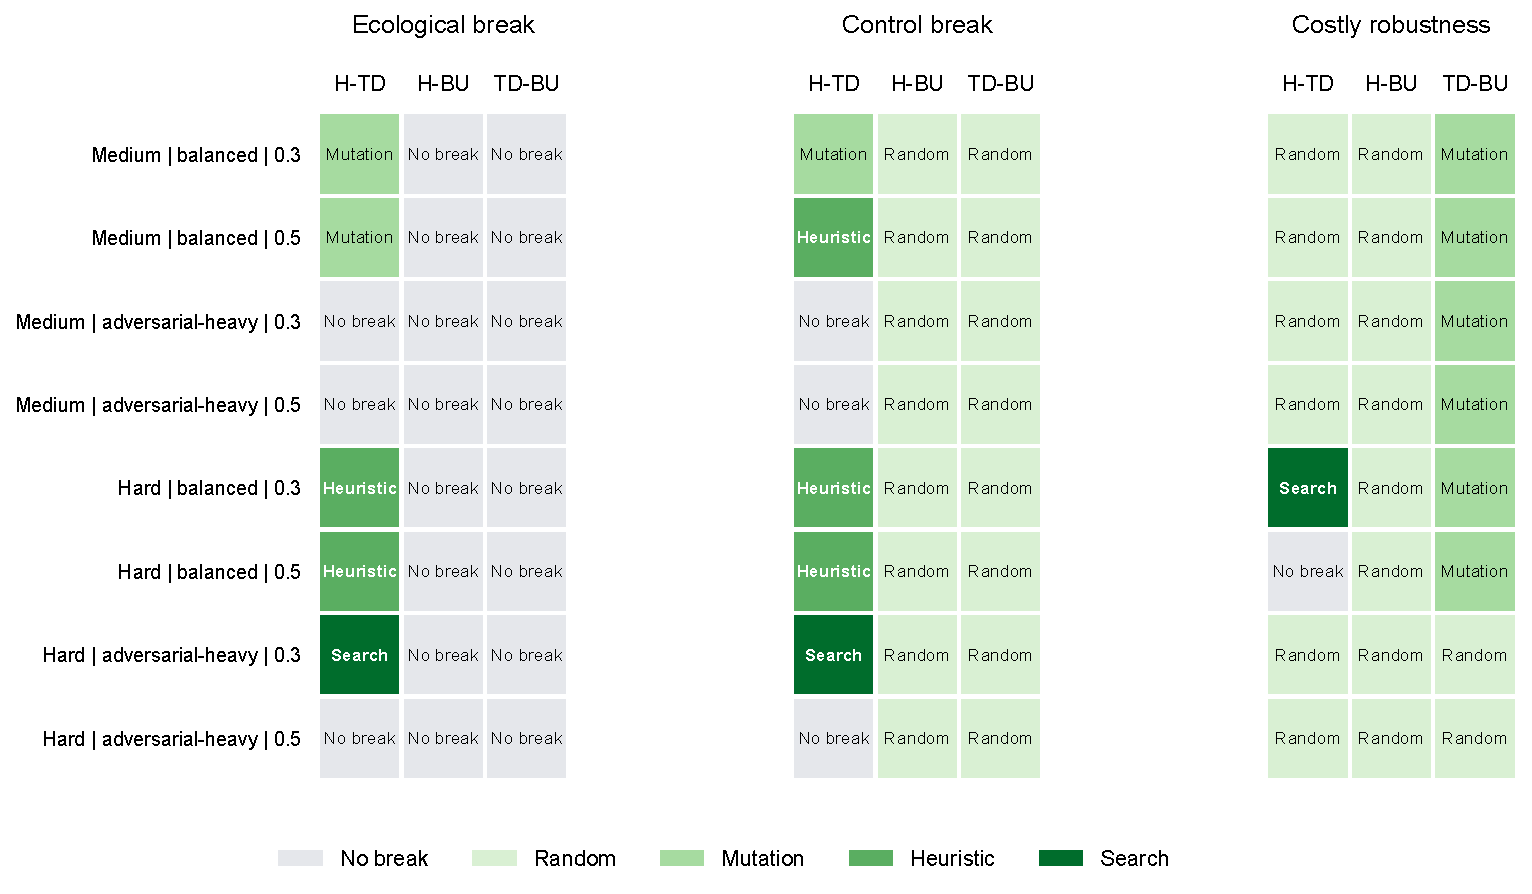
\includegraphics[width=\linewidth]{figures/harvest_capability_ladder_stageB_publication.pdf}
  \caption{Baseline Harvest capability ladder from the existing evidence base. The main split remains between architectures with central intervention and local-only governance, while the ordering between hybrid and top-down-only governance becomes more contested as attacker strength rises.}
  \label{fig:baseline_capability_ladder}
\end{figure}

\subsection{Architecture under institutional frictions}

Harvest is then re-evaluated under the three scenario archetypes and two oversight regimes. The main comparison remains hybrid versus top-down-only governance, with bottom-up-only governance retained as the decentralized comparison case.

The results vary across scenarios. In the community-irrigation scenario, hybrid governance ranks first in all four tested cells, under both ideal and constrained oversight, and records positive patch-health deltas against top-down-only governance in every case. In forest co-management, hybrid governance ranks first under ideal oversight, but top-down-only governance ranks first once oversight is constrained. In regulated fishery, the ranking depends on pressure: hybrid governance ranks first at the lower pressure level, whereas top-down-only governance ranks first at the higher pressure level in both oversight regimes.

Across all six scenario-pressure cells, the paired hybrid-minus-top-down-only contrast remains positive on patch health in five cells under ideal oversight and in five cells under constrained oversight. These ecological gains do not always translate into first-place ranking once welfare and control costs are included. Under ideal oversight, hybrid governance ranks first in five of the six cells. Under constrained oversight, it ranks first in three. The architecture ranking is therefore sensitive to scenario and oversight regime.

The decentralized baseline remains clearly weaker ecologically. Top-down-only governance exceeds bottom-up-only governance on patch health in every evaluated cell, and hybrid governance does the same. The cost of that ecological improvement is lower welfare relative to bottom-up-only governance, which remains the highest-welfare but least robust architecture. Figure~\ref{fig:moduleA_winner_map} summarizes the extension in a single winner map. Each cell shows the best-ranked architecture, while the annotated number reports the hybrid-minus-top-down patch-health difference.

\begin{figure}[t]
  \centering
  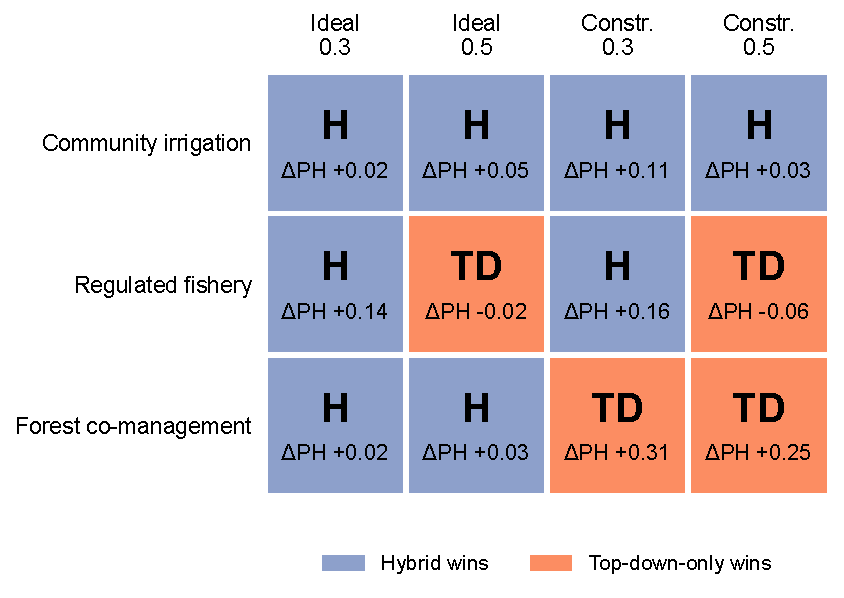
\includegraphics[width=0.88\linewidth]{figures/institutional_friction_winner_map.pdf}
  \caption{Compact summary of the institutional-friction extension. Cell color denotes the best-ranked architecture in each scenario, oversight regime, and pressure cell. The annotation reports the hybrid-minus-top-down patch-health difference, which shows where hybrid retains an ecological advantage even when it is not the overall winner.}
  \label{fig:moduleA_winner_map}
\end{figure}

\subsection{Scenario-Dependent Ranking}

The earlier confirmatory Harvest result showed that hybrid governance could outperform central-only control under stronger search-based pressure. The institutional-friction extension retains that result in some settings and reverses it in others. Once scenario structure and implementation frictions are introduced, the ordering between hybrid and top-down-only governance differs across cases. The resulting architecture ranking is scenario dependent.
